\chapter{Programmbeschreibung}\label{pro:ch:programmbeschreibung}

\section{Struktogramme}\label{pro:sec:pap}

\subsection{UML-Klassendiagramm}\label{pro:subsec:uml-klassendiagramm}
\begin{center}
    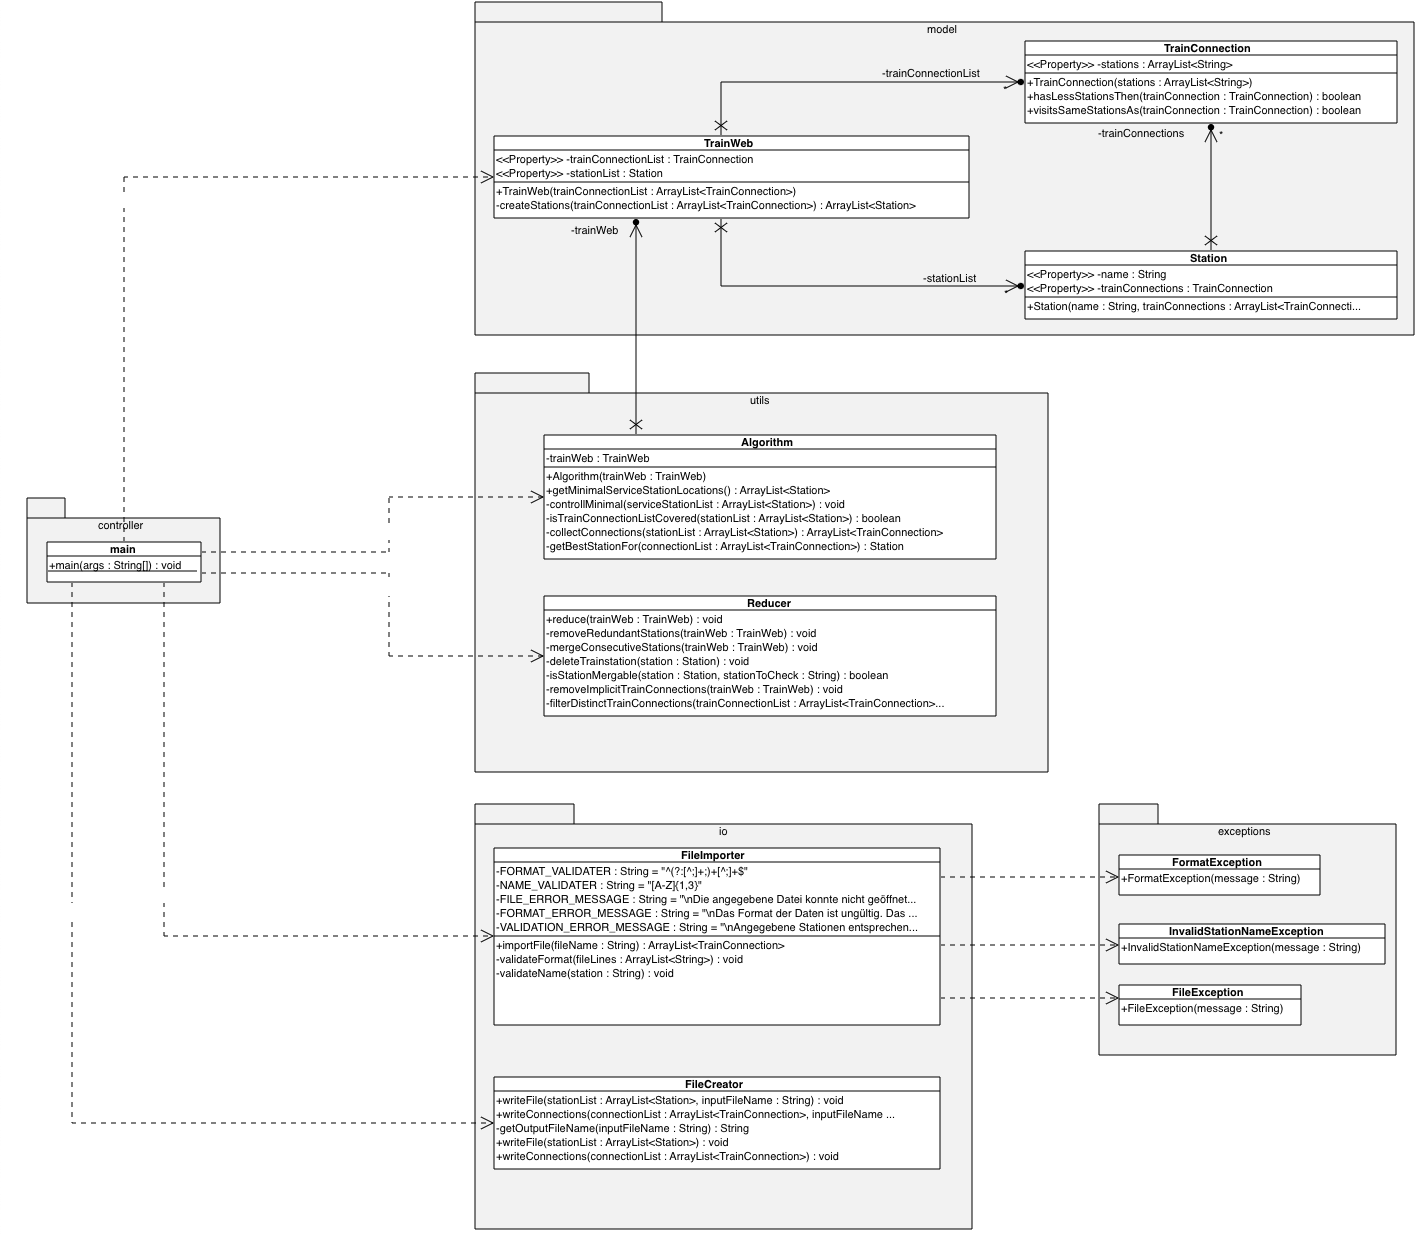
\includegraphics[width=\linewidth]{images/Struktogramme/UML-Klassendiagramm.png}
    \captionof{figure}{UML-Klassendiagramm}
    \label{pro:subsecpar:uml-klassendiagramm}
\end{center}

\subsection{UML-Sequenzdiagramm}\label{pro:subsec:uml-sequenzdiagramm}
\begin{center}
    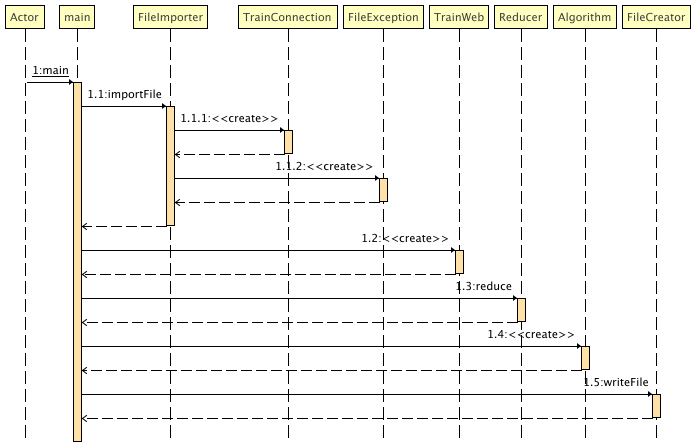
\includegraphics[width=\linewidth]{images/Struktogramme/Sequenzdiagramm.png}
    \captionof{figure}{UML-Sequenzdiagramm}
    \label{pro:subsecpar:uml-sequenzdiagramm}
\end{center}

\newpage
\subsection{Nassi-Shneiderman-Diagramme}\label{pro:subsec:nassi-shneiderman-diagramme}
\subsubsection{Input / Output}\label{pro:subsubsec:io}
\paragraph{Input}\label{pro:subsubsecpar:input}
\begin{center}
    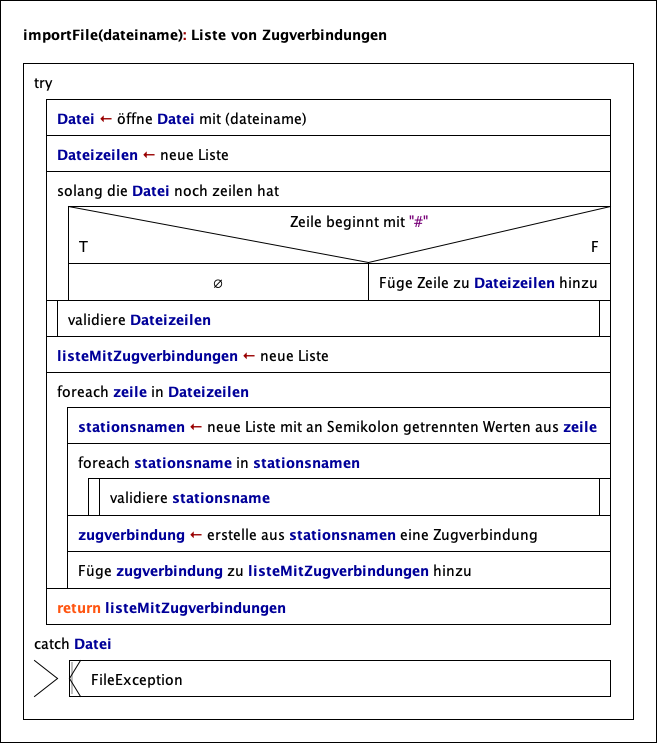
\includegraphics[width=\linewidth]{images/Struktogramme/io/importFile.png}
    \captionof{figure}{Input}
    \label{pro:subsubsecpar:inputFile}
\end{center}

\begin{center}
    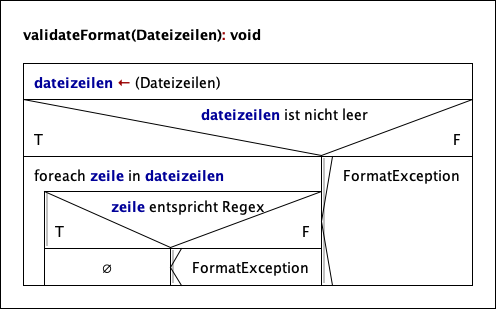
\includegraphics[width=\linewidth]{images/Struktogramme/io/validateFormat.png}
    \captionof{figure}{Format Validator}
    \label{pro:subsubsecpar:format-validator}
\end{center}

\begin{center}
    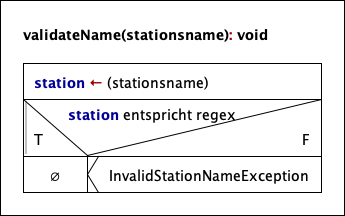
\includegraphics[width=\linewidth]{images/Struktogramme/io/validateName.png}
    \captionof{figure}{Namen Validator}
    \label{pro:subsubsecpar:namen-validator}
\end{center}


\paragraph{Output}\label{pro:subsubsecpar:output}
\begin{center}
    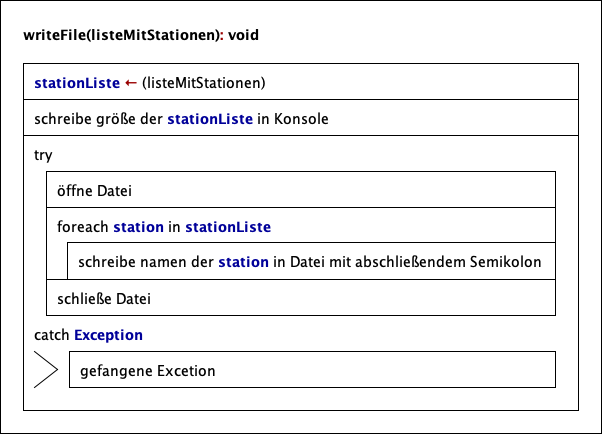
\includegraphics[width=\linewidth]{images/Struktogramme/io/writeFile.png}
    \captionof{figure}{Namen Validator}
    \label{pro:subsubsecpar:namen-validator}
\end{center}


\newpage
\subsubsection{Reduzieren}\label{pro:subsubsec:reduzieren}
\paragraph{Doppelstationen}\label{pro:subsubsubsec:doppelstationen}
\begin{center}
    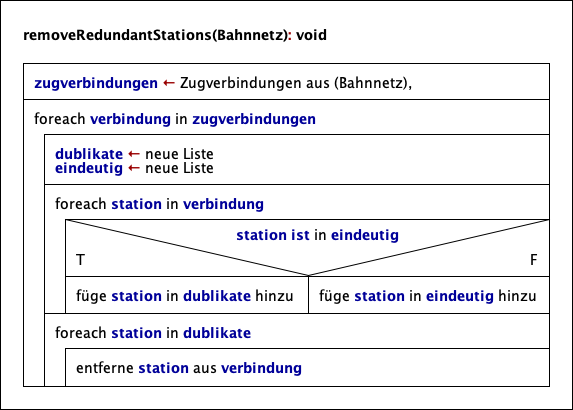
\includegraphics[width=\linewidth]{images/Struktogramme/reducer/reduction1/removeRedundantStations.png}
    \captionof{figure}{Entfernen von Doppelstationen}
    \label{pro:subsubsecpar:entfernen-von-doppelstationen}
\end{center}


\paragraph{Stationsabhängigkeiten}\label{pro:subsubsubsec:stationsabhaengigkeiten}
\begin{center}
    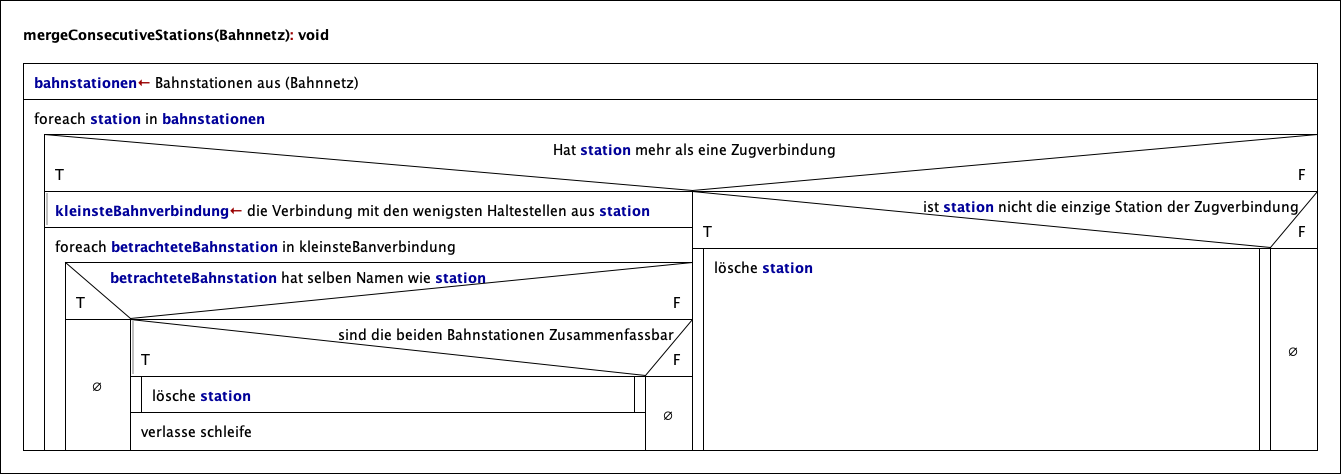
\includegraphics[width=\linewidth]{images/Struktogramme/reducer/reduction2/mergeConsecutiveStations.png}
    \captionof{figure}{Zusammenfassen von Stationen}
    \label{pro:subsubsecpar:zusammenfassen-von-stationen}
\end{center}

\begin{center}
    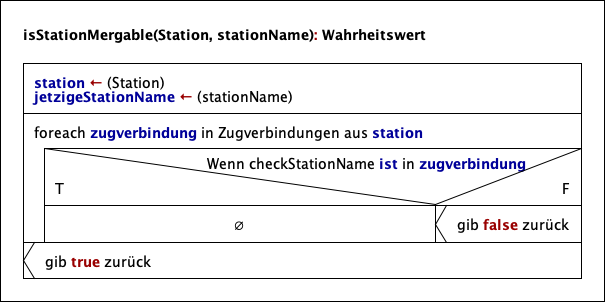
\includegraphics[width=\linewidth]{images/Struktogramme/reducer/reduction2/isStationMergable.png}
    \captionof{figure}{Überprüfung ob Stationen zusammenfassbar sind}
    \label{pro:subsubsecpar:ueberpruefung-ob-stationen-zusammenfassbar-sind}
\end{center}

\begin{center}
    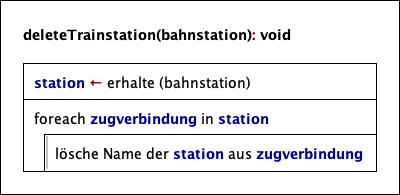
\includegraphics[width=\linewidth]{images/Struktogramme/reducer/reduction2/deleteTrainstation.png}
    \captionof{figure}{Entfernen von Stationen}
    \label{pro:subsubsecpar:entfernen-von-stationen}
\end{center}


\paragraph{Implizite Zugverbindungen}\label{pro:subsubsubsec:implizite-zugverbindungen}
\begin{center}
    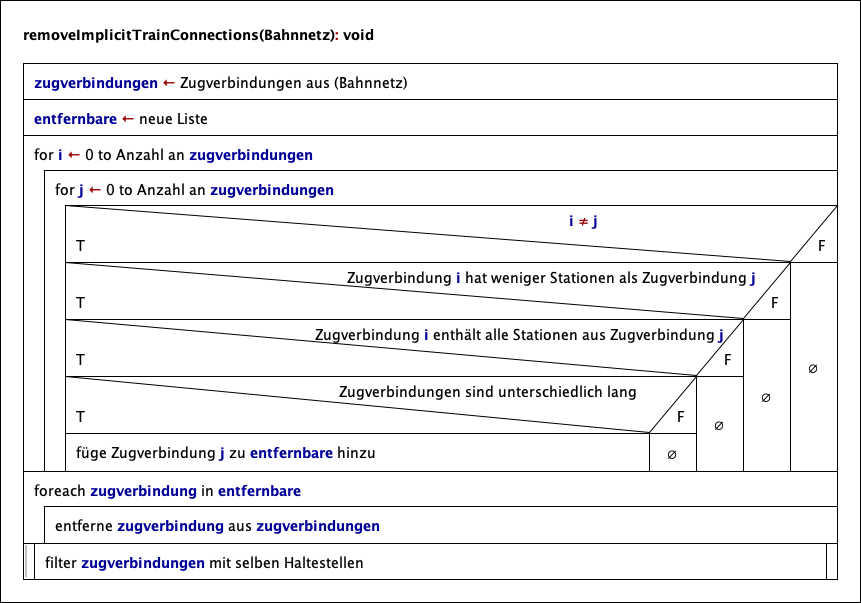
\includegraphics[width=\linewidth]{images/Struktogramme/reducer/reduction3/removeImplicitTrainConnections.png}
    \captionof{figure}{Entfernen von impliziten Zugverbindungen}
    \label{pro:subsubsecpar:entfernen-von-impliziten-zugverbindungen}
\end{center}

\begin{center}
    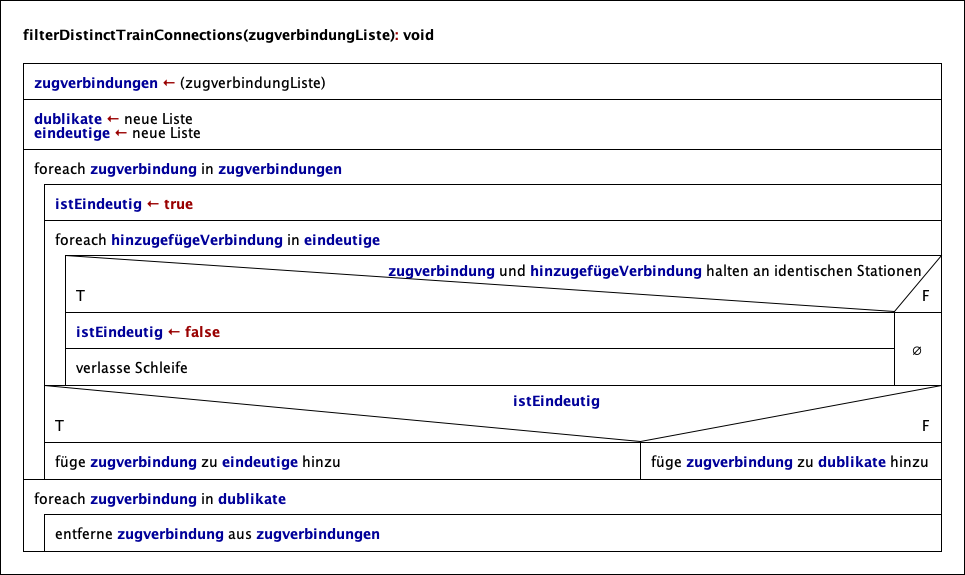
\includegraphics[width=\linewidth]{images/Struktogramme/reducer/reduction3/filterDistinctTrainConnections.png}
    \captionof{figure}{Entfernen von identischen Zugverbindungen}
    \label{pro:subsubsecpar:ueberpruefung-ob-zugverbindung-implizit-ist}
\end{center}

\newpage
\subsubsection{Algorithmus}\label{pro:subsubsec:algorithmus}
\begin{center}
    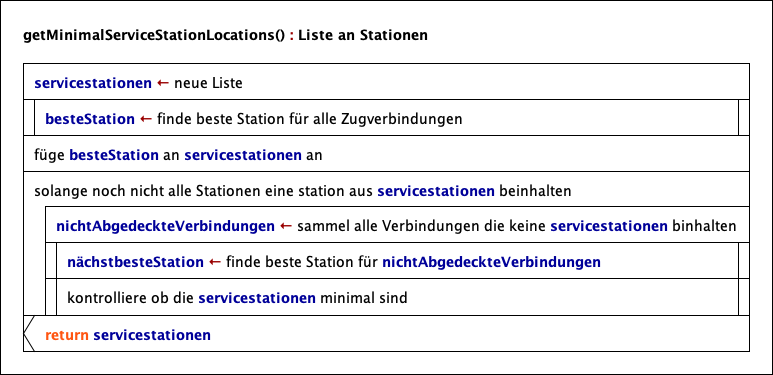
\includegraphics[width=\linewidth]{images/Struktogramme/algorithm/getMinimalServiceStationLocations.png}
    \captionof{figure}{Berechne minimale Anzahl an Servicestationen}
    \label{pro:subsubsecpar:berechne-minimale-anzahl-an-servicestationen}
\end{center}

\begin{center}
    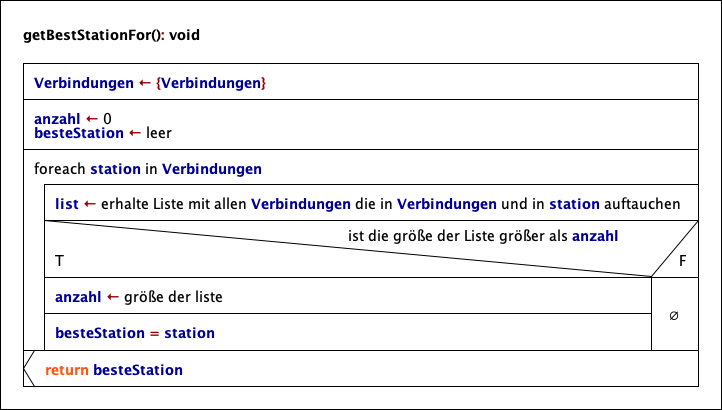
\includegraphics[width=\linewidth]{images/Struktogramme/algorithm/getBestStationFor.png}
    \captionof{figure}{Berechne beste Station für übergebene Zugverbindungen}
    \label{pro:subsubsecpar:berechne-minimale-anzahl-an-servicestationen}
\end{center}

\begin{center}
    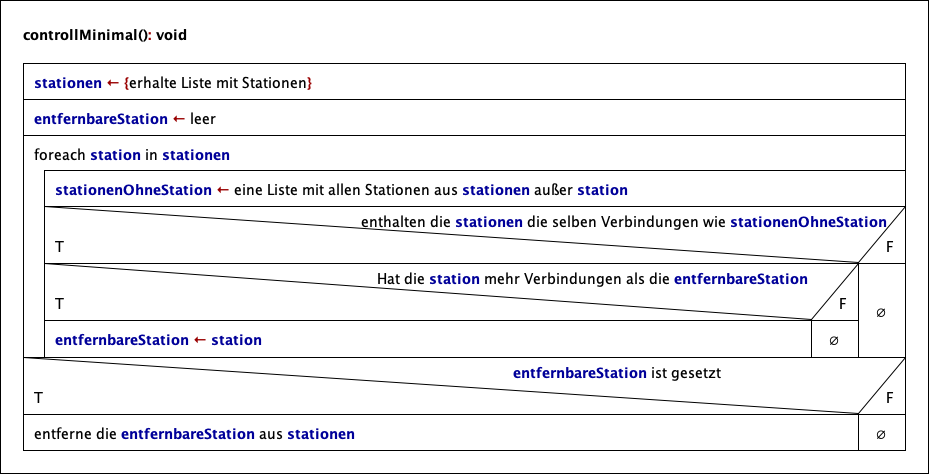
\includegraphics[width=\linewidth]{images/Struktogramme/algorithm/controllMinimal.png}
    \captionof{figure}{Überprüfe minimale Anzahl an Servicestationen}
    \label{pro:subsubsecpar:ueberpruefe-minimale-anzahl-an-servicestationen}
\end{center}

\section{Entwicklungsdokumentation}\label{pro:sec:entwicklerdokumentation}
Die Dokumentation des Programms wurde in Javadoc vorgenommen und kann im Ordner javadoc eingesehen werden.
Hierzu kann die index.html aufgerufen werden